\skriptsection{DFT - Diskrete Fourier Transformation}{109}
\subsection{Definitionen}
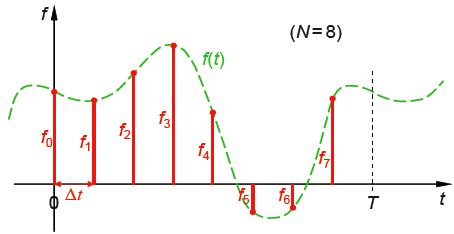
\includegraphics[width=5cm]{./bilder/abtastung.png}

\subsubsection{Diskrete komplexe Fourierkoeffizienten}
$\hat{c_k}$ sind die diskreten Fourierkoeffizienten die zu den (reellen
Abtastwerten $f_0, f_1,\ldots,f_{N-1}$) gehören\\
$$\hat{c_k}=\frac{1}{N}\sum\limits_{n=0}^{N-1}f_n\cdot e^{-\frac{2\pi j}{N}\cdot
kn}$$
Kompakte Darstellung mit der Matrix W:
$\begin{pmatrix}
 \hat{c_0}\\\hat{c_1}\\\hat{c_2}\\\hat{c_3}
\end{pmatrix}$
$=\frac{1}{N}$
$\begin{pmatrix}
 w^0w^0w^0w^0\\w^0w^1w^2w^3\\w^0w^2w^4w^6\\w^0w^3w^6w^9
\end{pmatrix}$
$\cdot$
$\begin{pmatrix}
 f_0\\f_1\\f_2\\f_3
\end{pmatrix}$
wobei $w=e^{-\frac{2\pi j}{N}}$

\subsubsection{Rechenaufwand DFT / FFT}
Der Rechenaufwand für die DFT ist proportional zu $N^2$ 
hingegen ist er bei der Fast Fourier Transform (FFT) nur $N\cdot log(N)$.

\skriptsubsection{Eigenschaften der Diskreten Fouriertransformation}{112}
\subsubsection{Alias-Effekt}
Mit $\hat{c_k}(\hat{c_0},\ldots,\hat{c_N-1})$ kennt man alle disktreten Fourierkoeffizienten. Es gilt:
$\hat{c_k}=\sum\limits_{l=-\infty}^{\infty}c_k+l\cdot N \quad l\in Z$

\subsubsection{Nyquist-Shannon-Abtasttheorem}
Ein Signal muss mit mindestens der doppelten Frequenz seines höchstfrequentigen Anteils abgetastet werden.

\skriptsubsection{Inverse Diskrete Fouriertransformation iDFT}{116}
\subsubsection{Abtastwerte berechnen}
Die N diskreten Fourierkoeffizienten lassen sich mit der iDFT wieder auf ihre Abtastwerte $f_n$ zurückführen.
$$f_n=\sum\limits_{k=0}^{N-1}(\hat{c_k}\cdot e^{\frac{2\pi j}{N}\cdot nk})$$
\subsubsection{Kontinuirliche Funktion berechnen}
Die N diskreten Fourierkoeffizienten lassen sich auch auf die kontinuirliche Funktion $f(t)$ zurückführen.
$$t\mapsto \sum\limits_{k=0}^{N-1}(\hat{c_k}e^{jk\omega_0t})$$ 
ist eine Funktion die diese diskreten Fourierkoeffizienten besitzt.
für $k=1,2,\ldots,\frac{N}{2}$ so ist auch 
$$t\mapsto\hat{c_k}+\sum\limits{k=1}{\frac{N}{2}-1}[2 
Re(\hat{c_k}e^jk\omega_0t)]+\hat{c_\frac{N}{2}}\cdot \cos(\frac{N}{2}\omega_0t)$$
eine reelle Funktion mit halb so grossen höchsten Frequenzen. 
